% SPDX-FileCopyrightText: 2023 SAP SE
%
% SPDX-License-Identifier: Apache-2.0
%
% This file is part of FEDEM - https://openfedem.org

%%%%%%%%%%%%%%%%%%%%%%%%%%%%%%%%%%%%%%%%%%%%%%%%%%%%%%%%%%%%%%%%%%%%%%%%%%%%%%%%
%
% FEDEM User Guide.
%
%%%%%%%%%%%%%%%%%%%%%%%%%%%%%%%%%%%%%%%%%%%%%%%%%%%%%%%%%%%%%%%%%%%%%%%%%%%%%%%%

\Chapter{Managing Results}{managing-results}

A Fedem simulation can generate large amounts of data.
This chapter explains the concept of the Fedem {\sl Results Data Base} (RDB),
how to manage the data files and some information on how Fedem stores and
handles the data.

Sections in this chapter address the following topics:

\begin{itemize}
\item
  \protect\hyperlink{model-and-result-file-handling}
                    {Model and Result file handling}
\item
  \protect\hyperlink{result-file-browser}
                    {Result File Browser}
\item
  \protect\hyperlink{rdb-directory-structure}
                    {RDB directory structure}
\end{itemize}

\clearpage


%%%%%%%%%%%%%%%%%%%%%%%%%%%%%%%%%%%%%%%%%%%%%%%%%%%%%%%%%%%%%%%%%%%%%%%%%%%%%%%%
\Section{Model and Result file handling}{model-and-result-file-handling}

A Fedem model consists of the mechanism model file, the FE-model files and all
the generated result data files. The generated results can be divided into
three main groups:

\begin{itemize}
\item FE-model reduction data
\item Dynamics response data
\item FE-recovery data
\end{itemize}

Normally all these groups can be looked upon as one single model even though it
is spread across several files and directories. Fedem keeps track of which files
that are part of your saved model and which are not.

Because the solvers write their data directly to disk while solving,
Fedem also tracks what files are part of your modified and unsaved model,
and can thus tell which files belong to the saved and the unsaved modified
version of your model.


\SubSection{Discarding unsaved changes}{discarding-unsaved-changes}

When you open an existing model, the original result files present on disk are
preserved, even if you delete results, change the model, run the solvers, etc.,
as long as you do not save your model. If you exit without saving,
all the original data remains unchanged and the result database will be restored
to the state of the last save.

The initial data is deleted or overwritten only when the model is saved.

Consequently, to be sure that the result files known by Fedem are those
(and only those) present on disk, the model has to be saved first.

\Note{If you use the Result File Browser to delete result files,
  they will be physically removed from disc instantly.
  Their removal will not be delayed until the first save.
  This is done to actually free disk space as you delete the files,
  and not when you save your model.}


\SubSection{Saving a model}{saving-a-model}

When the model is saved, the model file is updated with the current information
from memory, including information on the contents and status of the results
directory. In addition, all changed parts are saved in the FE model repository
(default: \File{link\_DB/} directory) and the obsolete files in the results
database are deleted.


%%%%%%%%%%%%%%%%%%%%%%%%%%%%%%%%%%%%%%%%%%%%%%%%%%%%%%%%%%%%%%%%%%%%%%%%%%%%%%%%
\Section{Result File Browser}{result-file-browser}

The Result File Browser is a dialog box that can be used to view and
manipulate files created by and used by the various Fedem modules.
It offers features such as enable and disable result files, and delete
individual results, or classes of results. It responds dynamically to
any changes in the results data base, and is kept up-to-date at all times.


\SubSection{The Result File Browser dialog}{the-result-file-browser-dialog}

\IconTextFirst{resultFileBrowser}{
  To open the Result File Browser dialog box,
  select \textbf{Result File Browser...} from the \textbf{Result} menu,
  or from the \textbf{Windows} tool bar.}

\noindent
\begin{picture}(344,220)
  \put(0,0){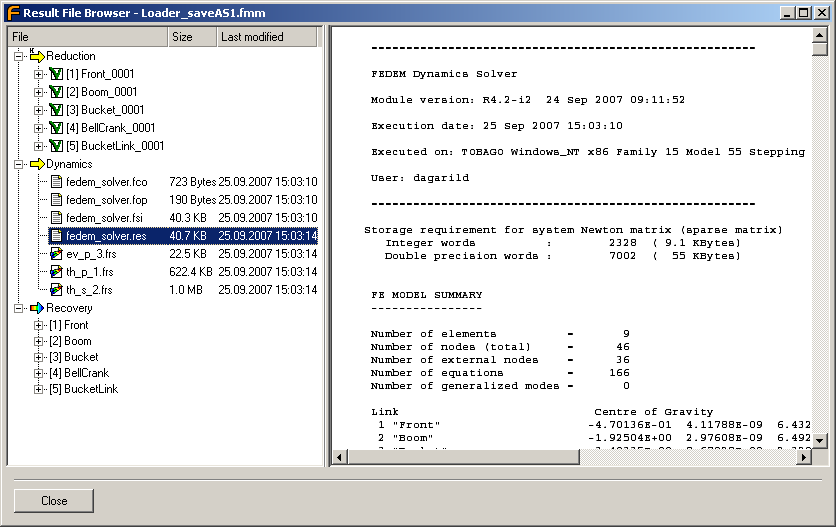
\includegraphics[width=\textwidth]{Figures/Dialogs/8-ResultFileBrowser}}
  \put(115,182){\Bullet{1}}
  \put(315,190){\Bullet{2}}
  \put(37,188){\Bullet{3}}
  \put(36,144){\Bullet{4}}
  \put(36,84){\Bullet{5}}
\end{picture}

\begin{bulletlist}
\item The {\sl File list} --
  Lists all relevant files from the {\sl Reduction},
  {\sl Dynamics} solver and {\sl Recovery} processes.
\item The {\sl Info view} --
  Displays information about the selected file.
\end{bulletlist}

\clearpage

\SubSubSection{The File list}{the-file-list}

The list is ordered chronologically,
with {\sl Reduction} first, then {\sl Dynamics} and {\sl Recovery}.
All directories will list the following file types, if present:

\begin{itemize}
\item\File{.frs} -- Binary result files
\item\File{.res} -- Log file for the solver processes
\item\File{.fco}, \File{.fop}, \File{.fao}, \File{.fsi} --
  Input files to the solver processes
\item\File{.fmx} -- Reducer matrix files
\item\File{.fsm} -- Internal data structure files
%\item\File{.fpp}, \File{.fef} -- Fatigue result files
\end{itemize}

The files are listed with file name, size and time of last modification.
Some of the files will also have an associated icon, corresponding to the icon
that file type will have in Windows Explorer.

When you run a solver process, the result files from it will appear in the file
list immediately after it is created, and it will be continuously updated up
until the process finishes.

\begin{bulletlist}
  \setcounter{enumi}{2}

\item{\sl Reduction} --
  This list shows the status and location of the results from the
  reduction process. The icon in front of each part indicates whether the part
  has a recognized set of reduced matrices or not.
  A green hatch indicates that the results are recognized as OK, a red cross
  indicates failure or that the part hasn't yet been reduced.

\item{\sl Dynamics} --
  Shows the result files produced by the Dynamics Solver.

\item{\sl Recovery} --
  Displays a list of all the parts in your model, and for each part the result
  files for that part grouped by the recovery process they were created by.
\end{bulletlist}

\Note{If you are working on a slow machine and have a lot of results displayed
  in the file list, continuously updating the list may steal valuable CPU cycles
  from the solver process. Close the Result File Browser dialog box to disable
  these updates and improve the overall performance.}

\clearpage

\subsubsection{The Info view}

When selecting a file in the file list, the file can be viewed in the info view.
The plain text files (\File{.fco}, \File{.fop}, \File{.fao}, \File{.fsi} and
\File{.res}) are displayed as-is, while selecting a \File{.frs} file will show
only the top of the header section.

Selecting a part under {\sl Reduction} will show information about that part,
as shown below.

\medskip\noindent
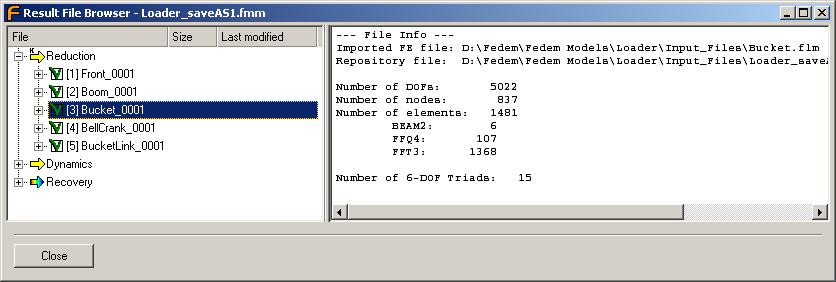
\includegraphics[width=\textwidth]{Figures/8-LinkFileInfo}

\medskip\noindent
In addition to the full path to the imported FE data file and the internal
repository file, you will here also get a summary of some size parameters
of the FE model for the part. This includes the total number of DOFs,
the number of nodes and the number elements of each type.
The number of triads attached to the part is also indicated.

The size information of the FE model is available also before the part
is reduced. It is therefore useful for assessing the computational cost
of reducing the part. This size information is not shown for Generic Parts,
even when a FE model is used for visualizing the part.


\SubSection{Result manipulation}{result-manipulation}

The Result File Browser can be used to manipulate the results,
both enable/disable results to decrease memory usage,
and delete single or multiple result files to save disk space.

\SubSubSection{Disabling and Enabling results}{disabling-and-enabling}

To disable/enable results, select the files you want to enable/disable,
right-click, and select either \textbf{Enable Results} or
\textbf{Disable Results} from the menu, as shown below. The icons of
the files immediately changes to reflect the current result state.

\begin{wrapfigure}[10]{r}{0.4\textwidth}
  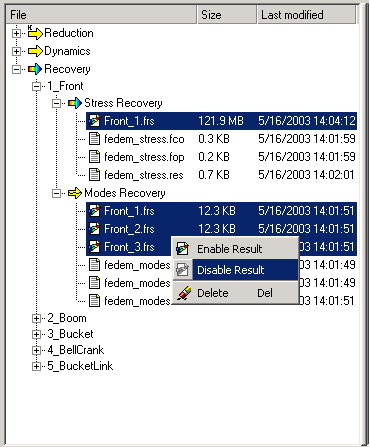
\includegraphics[width=0.4\textwidth]{Figures/RFB-disable}
\end{wrapfigure}

What you actually do when you disable a result file, is to temporarily remove
all result information in the file from memory, and the results from that file
will be unavailable for post-processing (curve plotting and animation).
As a result, Fedem will consume less memory.
You may re-enable the disabled results any time you wish.
The results from this file will then be available for post-processing again.

\MiniGenericNote{note}{NOTE}{-26.2mm}{0.54}{0.21}{1.1}{
  Selecting a top level item in the file list will also automatically
  select any \File{.frs} files located below that item in the list.}

\subsubsection{Deleting results}

\begin{wrapfigure}[6]{r}{0.4\textwidth}
  \vspace{-5mm}
  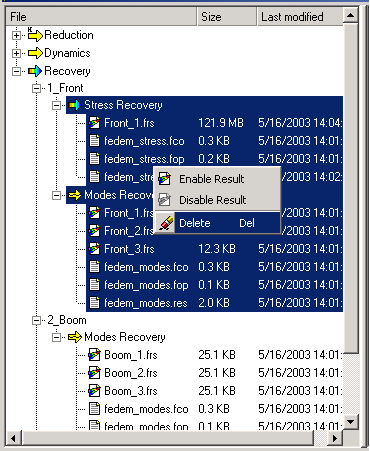
\includegraphics[width=0.4\textwidth]{Figures/RFB-delete}
\end{wrapfigure}

Using the same approach as when
\protect\hyperlink{disabling-and-enabling}{\sl Disabling and Enabling results},
you can also delete individual result files, classes of results,
or results on selected parts. Just select the results you want to delete,
right-click, and select \textbf{Delete} from the menu.

\MiniGenericNote{warning}{WARNING}{-26.2mm}{0.54}{0.21}{1.1}{
  Deleting the primary time history results (the file named \File{th\_p\_1.frs})
  will also cause all other results to be deleted.}

\MiniGenericNote{warning}{WARNING}{-26.2mm}{0.54}{0.21}{1.1}{
  When you delete results, they are physically removed from disc,
  and there is no way of getting them back at a later stage.
  An exception to this is when you delete the primary time history result file.
  In that case the results are not removed from disc until the next time
  you save your model.}


\SubSection{Result files from restart simulations}
           {result-files-from-restart-simulations}

When the Dynamics simulation has been restarted at least once
(see \refSubSection{time-tab}{Time tab}{dynamics-solver-advanced-mode}),
the {\sl Dynamics} part of \protect\hyperlink{the-file-list}{\sl The File list}
in the Result File Browser will contain solver option and result files for each
individual run. The option files (extension \File{.fop}, \File{.fco} and
\File{.fao}) and log-files (\File{.res}) from restart simulations will
have a number appended to the base name, indicating the actual restart number
(i.e., \File{fedem\_solver\_1.res}), whereas the binary result files
(\File{.frs}) will have numbers 3 or 4 and beyond, depending on whether
eigenmode analysis was activated.

\medskip\noindent
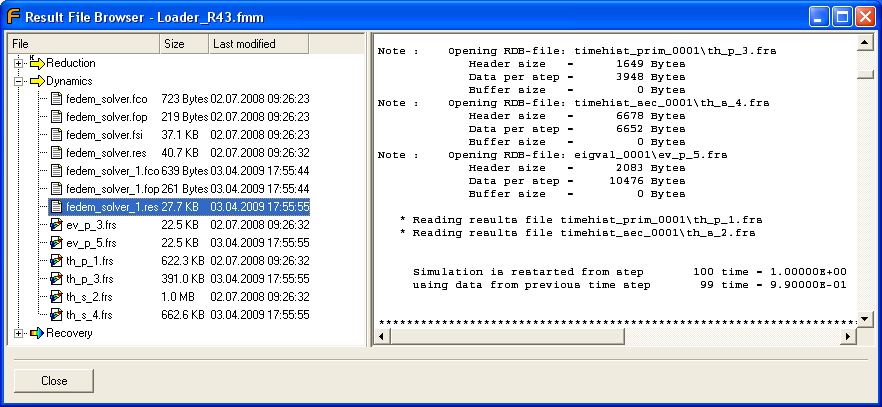
\includegraphics[width=\textwidth]{Figures/Dialogs/8-ResultFileBrowserRestart}

\medskip
\Note{There will always be only one \File{fedem\_solver.fsi} file in the
  File list regardless of whether results have been performed or not,
  because the same file is used by all restart runs. This file only contains
  model data that is not allowed to change in a restart.}

You may Enable/Disable and Delete individual files from restarts
in a similar way as the files from the original run
(see \refSection{result-manipulation}{Result manipulation}), in order to control
what results should be active for further post-processing and recovery runs.
If multiple results are active for a given time set of time steps,
only those that were produced latest will be used\footnote{
The same is true when post-processing results from recovery simulations that
have been rerun several times on the same dynamics simulation results.}.

\Note{If deleting a primary time history results file from a restart simulation
  (e.g., the file \File{th\_p\_3.frs} in the view above), all other simulation
  results are not automatically deleted as well, as happens when the primary
  result file of the original simulation, \File{th\_p\_1.frs}, is deleted).}


%%%%%%%%%%%%%%%%%%%%%%%%%%%%%%%%%%%%%%%%%%%%%%%%%%%%%%%%%%%%%%%%%%%%%%%%%%%%%%%%
\Section{RDB directory structure}{rdb-directory-structure}

The map below outlines the RDB directory structure created by Fedem.
The hierarchy root is named \File{[modelname]\_RDB}, where \File{[modelname]}
is the name of the current model. For example, the model file
\File{FrontSuspension.fmm} creates a results directory structure under
the directory \File{FrontSuspension\_RDB}.

\noindent\hspace{-12mm}
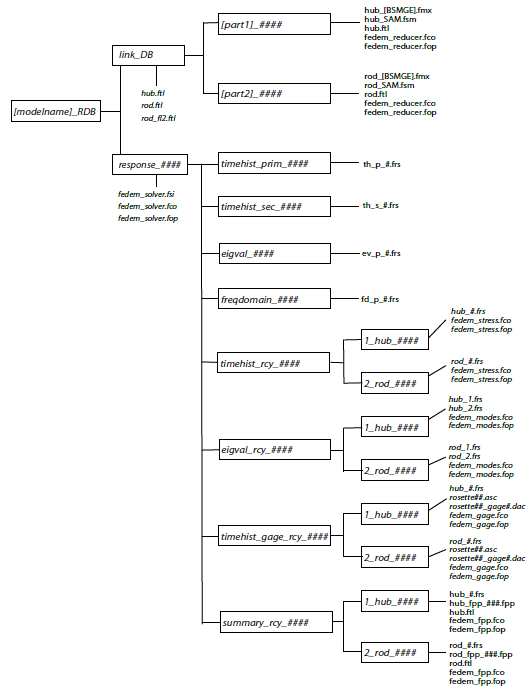
\includegraphics[height=\textheight]{Figures/8-RDB_DirectoryStructure}


\SubSection{Part database}{part-database}
\def\Hashes{\#\#\#\#}

The \File{link\_DB} directory (either specified as default, part-specific or
model-specific) contains Fedem \File{.ftl} files of all unique parts imported
into the Fedem model. All \File{.ftl} files in this directory are stored
without external node information. This reduces the total storage requirements.

A set of new subdirectories is created under the \File{link\_DB} directory to
store information about already reduced parts. This directory is named
\File{[partname]\_\Hashes}, where \File{[partname]} is the name of
the actual part, and \File{\Hashes} represents a configuration number.

Option files for Fedem Reducer are also stored in the \File{[partname]\_\Hashes}
directories. This enables reduced parts to be moved between result databases.

\Note{When a part- or model-specific repository is used
  (see \refSection{using-fe-model-repositories}{Using FE model repositories}),
  the file name conventions apply to the subdirectories of that directory,
  and not the \File{link\_DB} directory.}

\Caution{If you use a file browser to remove unwanted files in the Fedem Results
  Database directory structure, do not remove the \File{.ftl} files directly
  under the \File{link\_DB} directory. However, all other files will be
  automatically recreated when a new simulation starts.}

\Caution{If you use a file browser to move a Fedem Mechanism Model file
  (\File{.fmm}), you must also move the \File{link\_DB} directory
  to ensure inclusion of the part definitions.}

\subsubsection{Model reduction file management}

When the model reduction process is started,
a new directory for each FE part is created and the files needed by the
\File{fedem\_reducer} process are written to this directory.
These files include an \File{.ftl} file with external node specification,
and the options files \File{.fco}, \File{.fop} and \File{.fao}
(see \refSection{file-types}{File types}).

After the reduction, all input files are retained for reference and a
possible rerun of the process in batch mode at a later stage.


\SubSection{Response directory structure}{response-directory-structure}

The \File{response\_\Hashes} directory is the entry-point to result files from
dynamics simulation and recovery operations. Option files for the dynamics
solver are stored directly in the \File{response\_\Hashes} directory.
These files can be used to run the solver in batch mode.

\Caution{These files are auto-generated from the Fedem GUI application.
  Manually changing the contents of these files and running the solver from the
  command line creates results that are inconsistent with the definitions
  in the model file.}

All results files in the \File{response\_\Hashes} structure are stored in the
same format, but are placed in different directories, making separate result
types easily distinguishable.

The recovery modules will store their results in a part-wise manner in
subdirectories under their main result directory, named
\File{[ID]\_[partname]\_\Hashes}, where \File{[ID]} is the part identification
number. All option files are also stored in these subdirectories.

The following lists the result directories with descriptions of their contents:

\begin{itemize}

\item\File{timehist\_prim\_\Hashes} :
  The primary time history result files are named \File{th\_p\_\#.frs}
  and contain primary response results from the dynamics solver.

\item\File{timehist\_sec\_\Hashes} :
  The secondary time history result files are named \File{th\_s\_\#.frs}
  and contain all secondary response results from the dynamics solver.

\item\File{eigval\_\Hashes} :
  Calculated eigenvalues and associated eigenvectors from the
  dynamics simulation are stored in files named \File{ev\_\#.frs}.

\item\File{freqdomain\_\Hashes} :
  Results from the frequency response analysis are stored in files named
  \File{fd\_p\_\#.frs}. The result variables stored here might be in conflict
  will similar quantities in the \File{th\_p\_\#.frs} files,
  so make sure only one of them are active in the
  \protect\hyperlink{result-file-browser}{\sl Result File Browser}
  when viewing the results.

\item\File{timehist\_rcy\_\Hashes} :
  Results from the stress recovery process will be stored part-wise
  in subdirectories. The files will be named \File{[partname]\_\#.frs}.

\item\File{eigval\_rcy\_\Hashes} :
  Results from the eigenvalue recovery process will be stored part-wise
  in subdirectories under this directory,
  and will be named \File{[partname]\_\#.frs}.

\item\File{timehist\_gage\_\Hashes} :
  Results from strain rosette recovery are stored part-wise in subdirectories
  under this directory. The files will be named \File{[partname]\_\#.frs}.
  Fedem will also create ASCII and DAC files.
  See \refSection{strain-rosette-analysis-1}{Strain rosette analysis}.

\item\File{summary\_rcy\_\Hashes} :
  Results from strain coat recovery are stored part-wise in subdirectories
  under this directory. The result files are named \File{[partname]\_\#.frs}.
\end{itemize}

\subsubsection{Strain Coat Recovery Summary file management}

When the Strain Coat Recovery process is started, a new directory called

\medskip
\File{response\_\Hashes/summary\_rcy\_\Hashes/[ID]\_[partname]\_\Hashes}

\medskip\noindent
is created, and the input files needed by \File{fedem\_fpp} are written to
this directory. This also include an \File{.ftl} file with Strain Coat elements,
in addition to the option files \File{.fco}, \File{.fop} and \File{.fao}.
The Strain Coat elements are of a non-structural type and do not
affect the FE model reduction results.

\Note{The \File{.ftl} file written to this directory is not necessarily
  identical to the corresponding file in the FE model repository, depending on
  whether the model has been saved since the strain coat elements were created.}
